\documentclass[11pt,aspectratio=169]{beamer} % 11pt is default
\usetheme{metropolis} % [progressbar=frametitle]
\setbeamercolor{background canvas}{bg=white}
\setbeamertemplate{caption}{\insertcaption} 
\setbeamersize{text margin left=2em,text margin right=2em}
\setbeamertemplate{frame footer}{\vspace{-5pt}}

\usepackage[round]{natbib}
\usepackage{amsmath}
\usepackage{mathtools}
\usepackage[group-minimum-digits=4,group-separator={,}]{siunitx}
\usepackage{graphicx}
\usepackage{wrapfig}
\usepackage{multimedia}

\usepackage{tikz}
\usetikzlibrary{backgrounds}
\usetikzlibrary{arrows,shapes}
\usetikzlibrary{tikzmark}
\usetikzlibrary{calc}
\usepackage[dvipsnames]{xcolor}

\usepackage[skins,theorems]{tcolorbox}
\usepackage{pdfpages}
\usepackage{colortbl}
\usepackage{changepage}
\usepackage{booktabs}
\usepackage{makecell}
\usepackage{setspace}
\usepackage{algorithm}
\usepackage[noend]{algpseudocode}
\usepackage{subcaption}
\usepackage[framemethod=TikZ]{mdframed}
\usepackage{xspace}

\usepackage{annotate-equations}

% Shortcut for beamer frames
\newcommand{\bframe}[2][c]{\begin{frame}[#1]{#2}}
\newcommand{\eframe}{\end{frame}} % \eframe causes problems for some reason

% Shortcut for bold text
\newcommand{\fat}[1]{\textbf{#1}}

% Boxing items on slide
\newcommand{\Cboxed}[2]{\colorlet{currentcolor}{.}{\color{#1}\fbox{\color{currentcolor}#2}}} %create coloured box around equation

% checkmark and xmark
\usepackage{pifont}
\newcommand{\cmark}{\ding{51}}%
\newcommand{\xmark}{\ding{55}}%

% Highlighting text in orange
\newcommand{\e}[1]{\alert{#1}}

% Underline
\newcommand{\uline}[1]{\underline{#1}}

% Include figure
\newcommand{\imgw}[2]{\includegraphics[width=#2\textwidth]{#1}} % \imgw{file}{height-scale}
\newcommand{\imgh}[2]{\includegraphics[height=#2\textheight]{#1}} % \imgh{file}{width-scale}

% Shortcut for latex commands
\newcommand{\blist}{\vspace{-3pt}\begin{list}{\raisebox{1pt}{\small$\bullet$}}{\leftmargin=13pt\itemsep=4pt}}
\newcommand{\blisttab}{\vspace{5pt}\blist}
\newcommand{\elisttab}{\end{list}}
\newcommand{\listtab}{\\[3pt] $\Rightarrow$ }
\newcommand{\elist}{\end{list}\vspace{5pt}}
\newcommand{\bblock}[1]{\metroset{block=fill}\begin{block}{#1}}
\newcommand{\eblock}{\end{block}}
\newcommand{\bmath}[1][0]{\begin{equation*}\hspace{#1em}}
\newcommand{\emath}{\end{equation*}}
\newcommand{\bcol}{\begin{columns}}
\newcommand{\col}[1]{\column{#1\textwidth}}
\newcommand{\tcol}[1]{\column[T]{#1\textwidth}}
\newcommand{\ecol}{\end{columns}}
\newcommand{\place}[4]{\begin{textblock}{#3}(#1,#2) #4 \end{textblock}} % \place{x}{y}{width}{text}
\newcommand{\placeframed}[4]{\place{#1}{#2}{#3}{\fbox{\parbox{#3em}{#4}}}}
\newcommand{\placeimg}[4]{\place{#1}{#2}{#3}{\imgw{#4}{1}}} % \placeimg{x}{y}{width}{file}
\newcommand{\videolink}[2]{\movie[externalviewer]{{\bf Video:} #1}{videos/#2}} % \videolink{title}{file}
\newcommand{\btab}[1]{\begin{tabular}{#1}}
\newcommand{\etab}{\end{tabular}}
\newcommand{\balgo}[2][1.3]{{#2:} \\[5pt] \begin{algorithmic}[1] \linespread{#1}\selectfont}
\newcommand{\ealgo}{\end{algorithmic}}
\renewcommand{\algorithmicloop}{\textbf{repeat:}}
\newcommand{\cred}{\cellcolor{red!25}}
\newcommand{\cgreen}{\cellcolor{green!25}}

% Shortcut for commonly used math symbols
\newcommand{\condpr}[2]{\text{Pr}\hspace{-1pt}\left\{ #1 \ \mid \ #2 \right\}}
\newcommand{\exarg}[2]{\mathbb{E}_{#1}\hspace{-2pt}\left[ #2 \right]}
\newcommand{\exnoarg}[1]{\mathbb{E}_{#1}}
\NewDocumentCommand\ex{ m g }{
	\IfNoValueTF{#2}{\exnoarg{#1}}{\exarg{#1}{#2}}
}
\newcommand{\der}[2]{\frac{\partial #1}{\partial #2}}
\newcommand{\stats}{\mathcal{S}}
\newcommand{\acts}{\mathcal{A}}
\newcommand{\rews}{\mathcal{R}}
\newcommand{\eps}{\mathcal{E}}
\newcommand{\ver}{\,\vert\,}
\newcommand{\vhat}{\hat{v}}
\newcommand{\qhat}{\hat{q}}
% \newcommand{\para}{\textbf{w}}
\newcommand{\feats}{\textbf{x}}
\newcommand{\elig}{\textbf{z}}
\newcommand{\gradient}{\nabla}
\newcommand{\outline}{Lecture Outline}
\newcommand{\reading}{Reading}
\newcommand{\h}[1]{\emph{#1}}

\emph
% \newcommand{\lindex}[1]{%
% 	\lowercase{\def\temp{#1}%
% 	\expandafter\index\expandafter{\temp}%
% }

\newcommand{\indx}[1]{\index{#1}}
\newcommand{\hind}[1]{\h{#1}\lindex{#1}}

% Set of real numbers
\newcommand{\R}{\mathbb{R}}
% Proportional to
% Transpose of a vector x
\newcommand{\vectranspose}[1]{#1^\top}
% Transpose of a matrix X
\newcommand{\mattranspose}[1]{#1^\top}
% Probability
\newcommand{\pr}{\text{Pr}}
% Conditional probability of x given y
\newcommand{\cpr}[2]{\pr( #1 \mid #2 )}
% x sampled according to probability distribution p
\newcommand{\sampled}[2]{#1 \sim #2}
% Assign value y to variable x
\newcommand{\assign}[2]{#1 \gets #2}
% Training data set
\newcommand{\data}{\mathcal{D}}
% Concatenation of inputs a, b, c, ...
\newcommand{\con}[1]{\langle #1 \rangle}
% array with bracket
\newcommand{\bra}[2]{\left[ \begin{array}{#1} #2 \end{array} \right]}
% Indicator function: returns 1 if x is true, otherwise returns 0
\newcommand{\ind}[1]{[#1]_1}

% common way of referring to places
\newcommand{\seehere}[1]{(\cref{#1})}

% shortcut text commands
\newcommand{\rl}{RL\xspace}
\newcommand{\marl}{MARL\xspace}
\newcommand{\ctde}{CTDE\xspace}
\newcommand{\sa}{single-agent\xspace}
\newcommand{\ma}{multi-agent\xspace}
\newcommand{\Ma}{Multi-agent\xspace}
\newcommand{\mas}{multi-agent system\xspace}
\newcommand{\stat}{stationarity\xspace}
\newcommand{\nonstat}{non-stationarity\xspace}
\newcommand{\pg}{policy gradient\xspace}
\newcommand{\vb}{value-based\xspace}
\newcommand{\pbt}{population-based training\xspace}
\newcommand{\psro}{policy space response oracles\xspace}
\newcommand{\Psro}{Policy space response oracles\xspace}
\newcommand{\sct}{\emph{StarCraft~II}\xspace}
\newcommand{\as}{AlphaStar\xspace}
\newcommand{\az}{AlphaZero\xspace}
\newcommand{\lbf}{level-based foraging\xspace}
\newcommand{\Lbf}{Level-based foraging\xspace}
\newcommand{\nfg}{normal-form game\xspace}
\newcommand{\nfgs}{normal-form games\xspace}
\newcommand{\Nfg}{Normal-form game\xspace}
\newcommand{\Nfgs}{Normal-form games\xspace}
\newcommand{\rps}{Rock-Paper-Scissors\xspace}
\newcommand{\pd}{Prisoner's Dilemma\xspace}
\newcommand{\survey}[4]{\noindent #1 (#4). ``#2.'' In: {\it #3}. \\}
\newcommand{\nashprob}{\textsc{Nash}\xspace}
\newcommand{\eol}{\textsc{End-of-Line}\xspace}
\newcommand{\ul}[1]{\underline{#1}}
\newcommand\norm[1]{\lVert#1\rVert}
\newcommand{\qlearn}{Q-learning\xspace}
\newcommand{\sarsa}{Sarsa\xspace}
\newcommand{\bayes}{Bayesian\xspace}
\newcommand{\bellman}{Bellman\xspace}
\newcommand{\markov}{Markov\xspace}
\newcommand{\pareto}{Pareto\xspace}
\newcommand{\boltzmann}{Boltzmann\xspace}
\newcommand{\mc}{Monte Carlo\xspace}
\newcommand{\nash}{Nash\xspace}
\newcommand{\ppad}{PPAD}
\newcommand{\dqn}{deep Q-networks\xspace}
\newcommand{\reinforce}{REINFORCE\xspace}
\newcommand{\qmix}{QMIX\xspace}
\newcommand{\qtran}{QTRAN\xspace}
\newcommand{\adam}{Adam\xspace}
\newcommand{\nret}{{$N$}-step returns\xspace}

% COMMANDS FOR COMMON NOTATION

% agent set
% state space
\newcommand{\St}{S}
\newcommand{\Stterm}{\bar{\St}}
% state
\newcommand{\st}{s}
\newcommand{\sth}{\hat{\st}}
% observation space
\newcommand{\Ob}{O}

% observation
\newcommand{\ob}{o}

% joint observation
\newcommand{\job}{o}
% action space
\newcommand{\Ac}{A}

% action
\newcommand{\ac}{a}
\newcommand{\ach}{\hat{\ac}}

% joint action
\newcommand{\jac}{a}
% reward
\newcommand{\rew}{r}
\newcommand{\rewh}{\hat{\rew}}
% centralised information
\newcommand{\ci}{z}

% initial state distribution

\newcommand{\instdist}{\mu}
% % state transition function

\newcommand{\Stf}{\mathcal{T}}
% % simulation/sampling model
\newcommand{\Stfsim}{\widehat{\Stf}}

% observation function
\newcommand{\Obf}{\mathcal{O}}

% reward function
\newcommand{\Rew}{\mathcal{R}}

% POLICIES, RETURNS, VALUES

% policy space
\newcommand{\Pol}{\Pi}

% policy
\newcommand{\pol}{\pi}
\newcommand{\poltil}{\tilde{\pol}}

% set of histories
\newcommand{\His}{H}
\newcommand{\Fhis}{\hat{\His}}
% history
\newcommand{\his}{h}

% full history
\newcommand{\fhis}{\hat{\his}}

% observation history extracted from full history
\newcommand{\obsext}{\sigma}

% discount factor
\newcommand{\dsc}{\gamma}

% return
\newcommand{\ret}{u}

% expected return for joint policy
\newcommand{\exret}{U}

% Agents
\newcommand{\Ag}{I}

% RL / MARL

% learning algorithm

\newcommand{\alg}{\mathbb{L}}

% empirical distribution/ average policy
\newcommand{\empdis}{\bar{\pol}}
\newcommand{\avgpol}{\bar{\pol}}
\newcommand{\agmod}{\hat{\pol}}
\newcommand{\Agmod}{\hat{\Pol}}
\newcommand{\agmodj}{agent model for agent $j$}

% best response
\newcommand{\br}{\textnormal{BR}}

% game value
\newcommand{\gval}{Value}

% value under agent model
\newcommand{\amval}{AV}

% regret
\newcommand{\regret}{Regret}
\newcommand{\avgreg}{\bar{R}}
% TD target
\newcommand{\target}{\mathcal{X}}
% step size (for gradient-based MARL in Chapter 5)
\newcommand{\step}{\kappa}


% DEEP LEARNING

% parameters
\newcommand{\para}{\theta}

% loss
\newcommand{\loss}{\mathcal{L}}
% batch
\newcommand{\batch}{\mathcal{B}}
\newcommand{\batchsize}{B}

% etnropy
\newcommand{\entropy}{\mathcal{H}}

% Create algorithm environment
\newcommand{\balg}[2]{
  \begin{algorithm}[H]
    \caption{#1}
    \label{alg:#2}
    \setstretch{1.1}
    \begin{algorithmic}[1]}

\newcommand{\ealg}{
    \end{algorithmic}
  \end{algorithm}}

% Argmin/ Argmax operators

\DeclareMathOperator*{\argmin}{arg\,min} 
\DeclareMathOperator*{\argmax}{arg\,max}

\makeatletter
\newenvironment{myitemize}{%
   \setlength{\topsep}{0pt}
   \setlength{\partopsep}{0pt}
   \renewcommand*{\@listi}{\leftmargin\leftmargini \parsep\z@ \topsep\z@ \itemsep\z@}
   \let\@listI\@listi
   \itemize
}{\enditemize}
\makeatother  

% define widebar for target parameters
\makeatletter
\newcommand*\rel@kern[1]{\kern#1\dimexpr\macc@kerna}
\newcommand*\widebar[1]{%
	\begingroup
	\def\mathaccent##1##2{%
		\rel@kern{0.8}%
		\overline{\rel@kern{-0.8}\macc@nucleus\rel@kern{0.2}}%
		\rel@kern{-0.2}%
	}%
	\macc@depth\@ne
	\let\math@bgroup\@empty \let\math@egroup\macc@set@skewchar
	\mathsurround\z@ \frozen@everymath{\mathgroup\macc@group\relax}%
	\macc@set@skewchar\relax
	\let\mathaccentV\macc@nested@a
	\macc@nested@a\relax111{#1}%
	\endgroup
}
\makeatother


% MATRIX GAMES

\newcolumntype{?}{!{\vrule width 1pt}}
\newcommand{\bhline}{\Xhline{1pt}}
\newcommand{\gametwo}[3]{
	\begin{tabular}{c?c|c}
		 & #1 \\
		\bhline
		#2    \\
		\hline
		#3    \\
	\end{tabular}
}
\newcommand{\gamethree}[4]{
	\begin{tabular}{c?c|c|c}
		 & #1 \\
		\bhline
		#2    \\
		\hline
		#3    \\
		\hline
		#4    \\
	\end{tabular}
}

\newcommand{\gamepd}{
    % \gametwo{C & D}{C & -1,-1 & -5,0}{D & 0,-5 & -3,-3}
	\begin{tabular}{c|c|c}
	& C & D \\
	\hline
	C & -1,-1 & -5,0 \\
	\hline
	D & 0,-5 & -3,-3
	\end{tabular}
}

\newcommand{\gamerps}{
    % \gamethree{R & P & S}{R & 0,0 & -1,1 & 1,-1}{P & 1,-1 & 0,0 & -1,1}{S & -1,1 & 1,-1 & 0,0}
	\begin{tabular}{c|c|c|c}
	& R & P & S \\
	\hline
	R & 0,0 & -1,1 & 1,-1 \\
	\hline
	P & 1,-1 & 0,0 & -1,1 \\
	\hline
	S & -1,1 & 1,-1 & 0,0
	\end{tabular}
}

\newcommand{\gamecoord}{
    % \gametwo{A & B}{A & 10 & 0}{B & 0 & 10}
	\begin{tabular}{c|c|c}
		& A & B \\
		\hline
		A & 10 & 0 \\
		\hline
		B & 0 & 10 \\
	\end{tabular}
}

\newcommand{\gamechicken}{
    % \gametwo{S & L}{S & 0,0 & 7,2}{L & 2,7 & 6,6}
	\begin{tabular}{c|c|c}
		& S & L \\
		\hline
		S & 0,0 & 7,2 \\
		\hline
		L & 2,7 & 6,6
	\end{tabular}
}

\newcommand{\gamestaghunt}{
    % \gametwo{S & H}{S & 4,4 & 0,3}{H & 3,0 & 2,2}
	\begin{tabular}{c|c|c}
		& S & H \\
		\hline
		S & 4,4 & 0,3 \\
		\hline
		H & 3,0 & 2,2
	\end{tabular}
}

\newcommand{\gamebattle}{
    \begin{tabular}{c|c|c}
    & A & B \\
    \hline
    A & 10,7 & 2,2 \\
    \hline
    B & 0,0 & 7,10
    \end{tabular}
}

\newcommand{\gameepsne}{
    % \gametwo{C & D}{A & 100,100 & 0,0}{B & 1,2 & 1,1}
	\begin{tabular}{c|c|c}
		& C & D \\
		\hline
		A & 100,100 & 0,0 \\
		\hline
		B & 1,2 & 1,1
	\end{tabular}
}

% Define colorboxes
\tcbset{
  % Defaults
  my box/main style/.style={},
  my box/title style/.style={},
  % Use the 'append' variants if you want to add to the defaults instead of
  % overriding them.
  my box/main/.style={/tcb/my box/main style/.style={#1}},
  my box/title/.style={/tcb/my box/title style/.style={#1}},
  my box/append main/.style={/tcb/my box/main style/.append style={#1}},
  my box/append title/.style={/tcb/my box/title style/.append style={#1}},
  %
  my box/.style={
    my box/.cd, #1,
    /tcb/.cd,
    enhanced,
    my box/main style,
    attach boxed title to top left={xshift=0.2cm, yshift=-0.2cm},
    top=10pt,
    boxed title style={
      outer arc=0pt,
      arc=0pt,
      top=3pt,
      bottom=3pt,
      my box/title style,
    },
  },
}

% define 'solutionbox' environment with coloured box
\newtcolorbox{solutionbox}[1][]{
  my box={
    main={colframe=green!40!gray!90, colback=green!20!gray!5},
    title={colback=green!40!gray!90},
  },
  title=Solution,
  #1,
}

\newtcolorbox{problembox}[1][]{
  my box={
    main={colframe=red!40!gray!90, colback=red!20!gray!5},
    title={colback=red!40!gray!90},
  },
  title=Problem,
  #1,
}

\newtcolorbox{notebox}[1][]{
  my box={
    main={colframe=orange!40!gray!80, colback=orange!20!gray!5},
    title={colback=orange!40!gray!80},
  },
  title=Note,
  #1,
}

\newtcolorbox{intuitionbox}[1][]{
  my box={
    main={colframe=blue!60!gray!80, colback=blue!20!gray!5},
    title={colback=blue!60!gray!80},
  },
  title=Intuition,
  #1,
}

\newtcolorbox{reminderbox}[1][]{
  my box={
    main={colframe=black!40!gray, colback=gray!10!white},
    title={colback=black!40!gray},
  },
  title=Reminder,
  #1,
}

\newtcolorbox{greentitlebox}[2][]{
  my box={
    main={colframe=green!40!gray!90, colback=green!20!gray!5},
    title={colback=green!40!gray!90},
  },
  title={#2},
  #1,
}

\newtcolorbox{redtitlebox}[2][]{
  my box={
    main={colframe=red!40!gray!90, colback=red!20!gray!5},
    title={colback=red!40!gray!90},
  },
  title={#2},
  #1,
}

\newtcolorbox{orangetitlebox}[2][]{
  my box={
    main={colframe=orange!40!gray!80, colback=orange!20!gray!5},
    title={colback=orange!40!gray!80},
  },
  title={#2},
  #1,
}

\newtcolorbox{bluetitlebox}[2][]{
  my box={
    main={colframe=blue!60!gray!80, colback=blue!20!gray!5},
    title={colback=blue!60!gray!80},
  },
  title={#2},
  #1,
}

\newtcolorbox{graytitlebox}[2][]{
  my box={
    main={colframe=black!40!gray, colback=gray!10!white},
    title={colback=black!40!gray},
  },
  title={#2},
  #1,
}

% no title boxes
\newtcolorbox{greenbox}[1][]{
  my box={
    main={colframe=green!40!gray!90, colback=green!20!gray!5},
  },
  #1,
}
\newtcolorbox{redbox}[1][]{
  my box={
    main={colframe=red!40!gray!90, colback=red!20!gray!5},
  },
  #1,
}
\newtcolorbox{orangebox}[1][]{
  my box={
    main={colframe=orange!40!gray!80, colback=orange!20!gray!5},
  },
  #1,
}
\newtcolorbox{bluebox}[1][]{
  my box={
    main={colframe=blue!60!gray!80, colback=blue!20!gray!5},
  },
  #1,
}
\newtcolorbox{blackbox}[1][]{
  my box={
    main={colframe=black!55!black, colback=gray!5!white},
  },
  #1,
}


% Define intro slide command
\newcommand{\introslide}{
    \begin{frame}[t]{The MARL Book}
        \bcol           
            \col{0.54}
	        	\small
                This lecture is based on \\[5pt]
                \textbf{Multi-Agent Reinforcement Learning: Foundations and Modern Approaches} \\[5pt]
                by Stefano V. Albrecht, Filippos Christianos and Lukas Sch\"afer \\[5pt]
                MIT Press, 2024
                
                \vspace{20pt}

				\centering
                
                Download book, slides, and code at:

                \textcolor{blue}{\href{https://www.marl-book.com/}{\bf www.marl-book.com}}
                
            \col{0.4}
	            \vspace{5pt}
	            
	            \centering
	            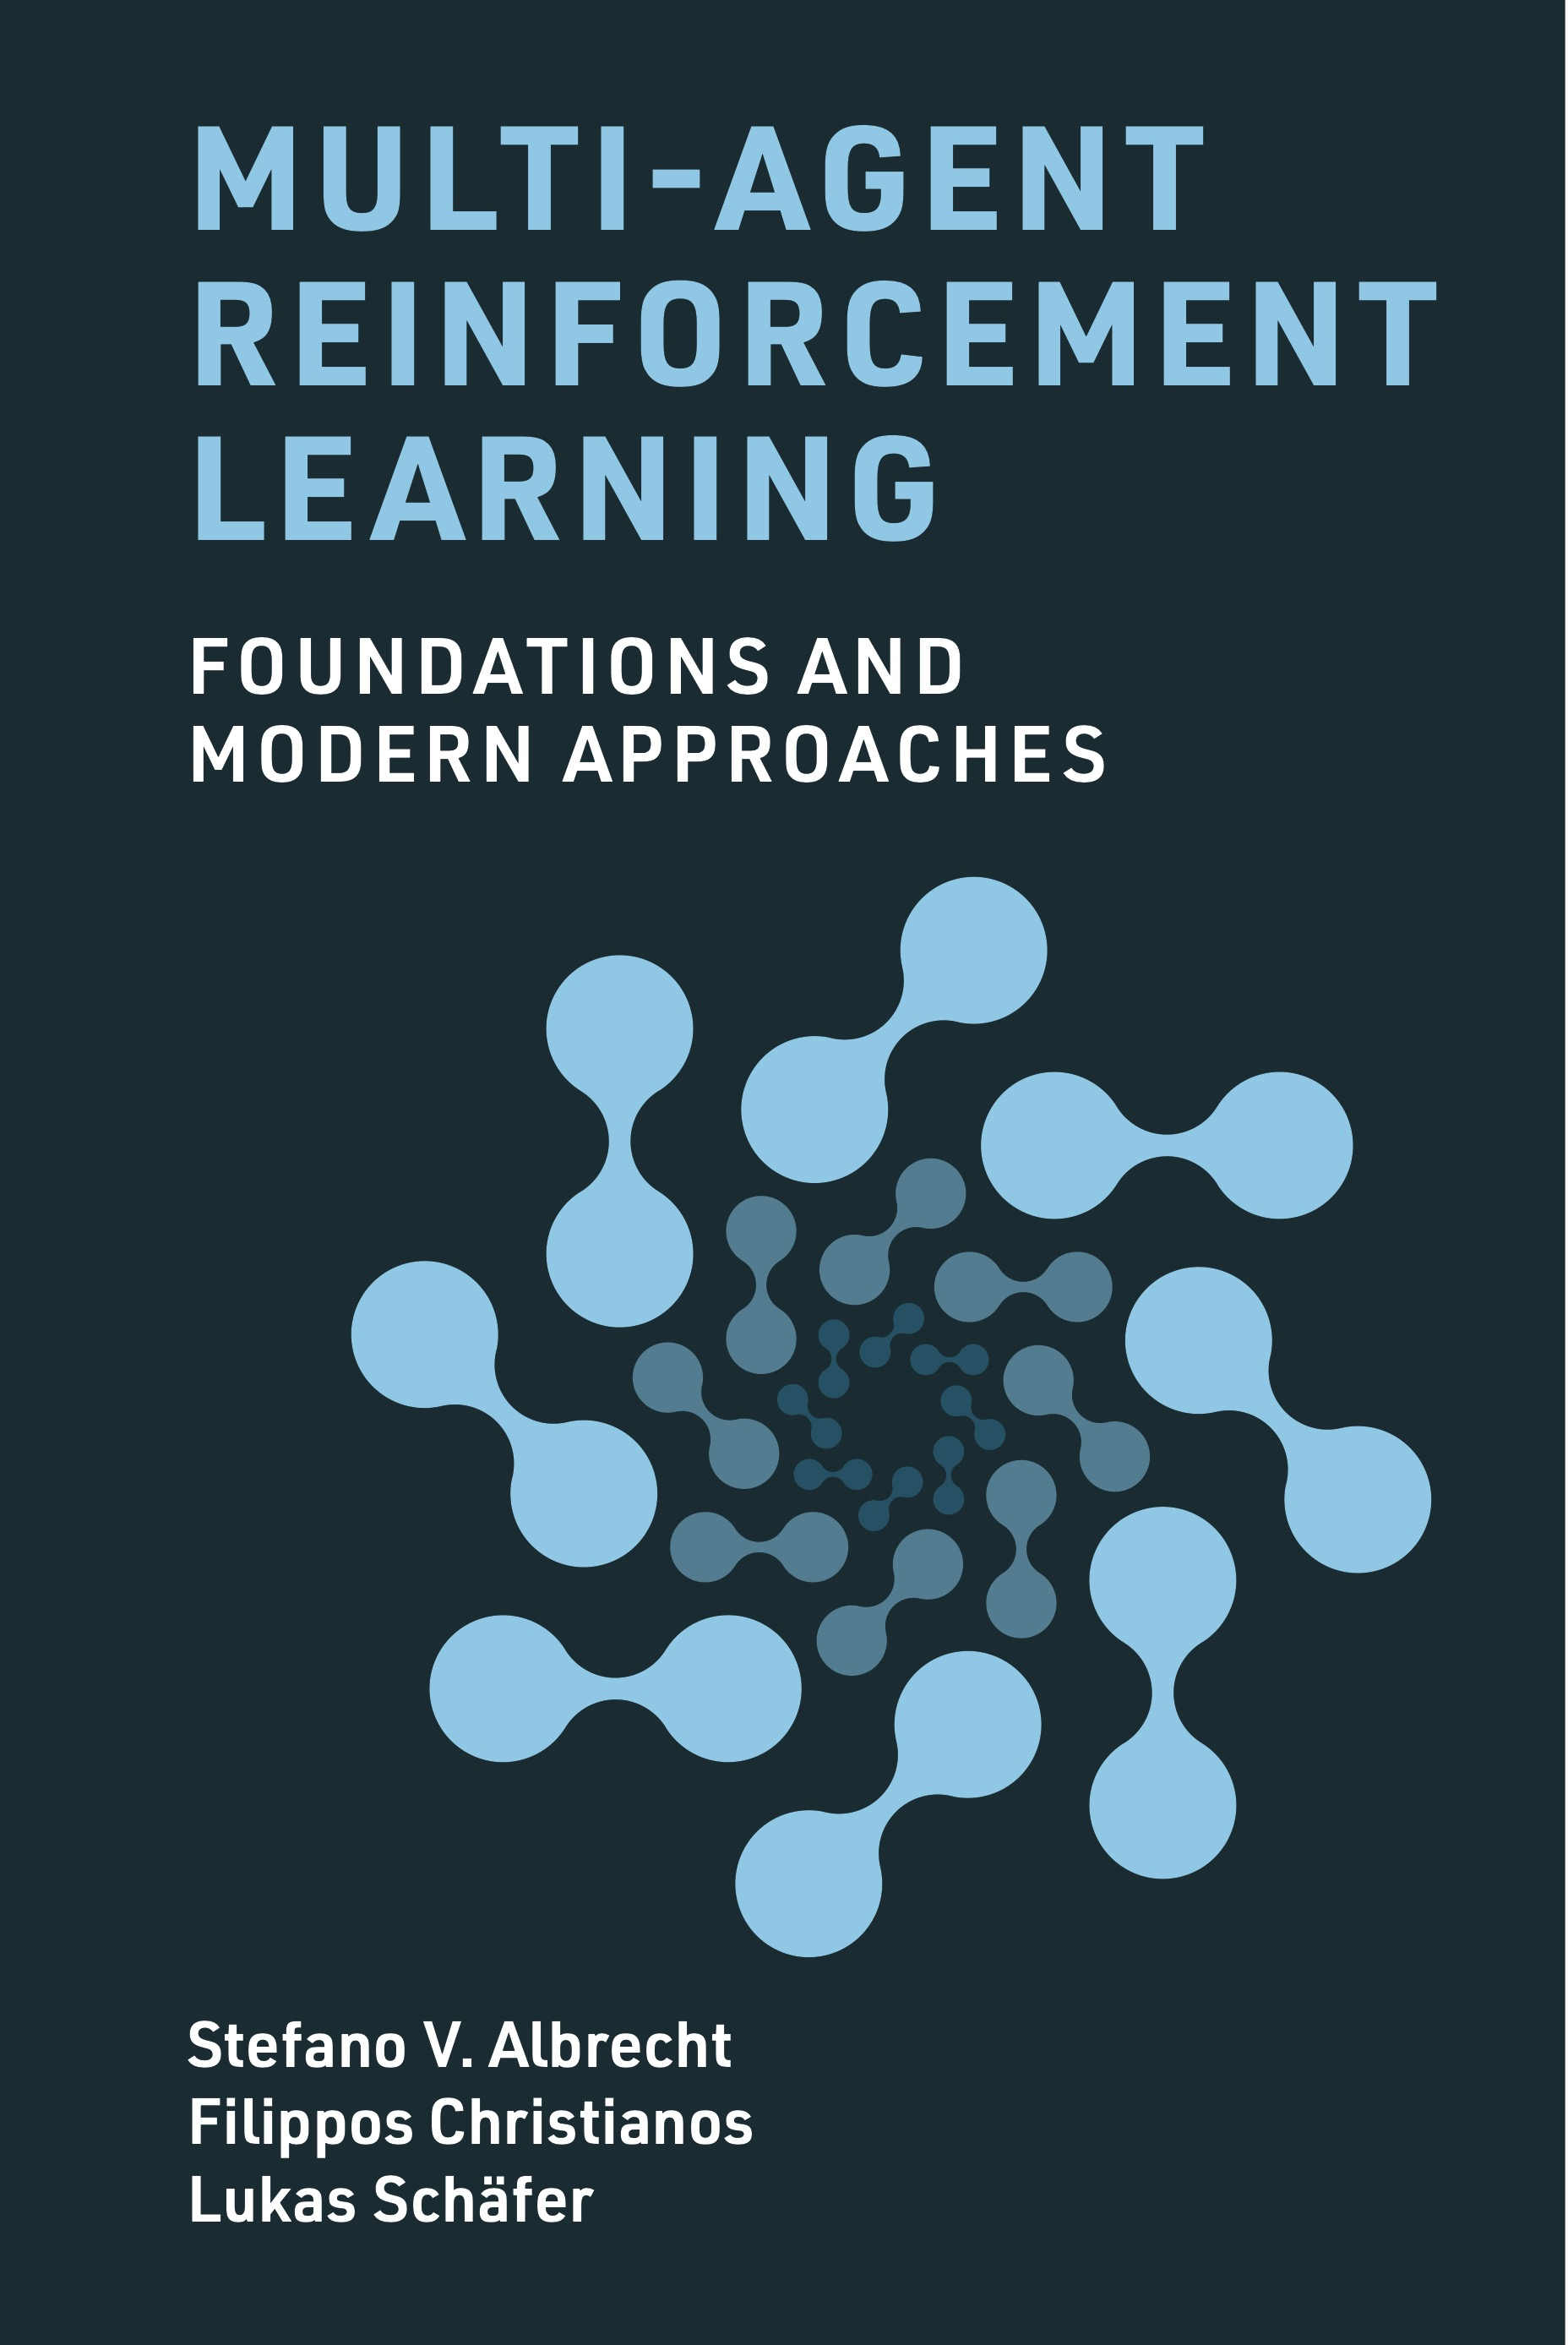
\includegraphics[width=0.82\textwidth]{images/marl-book-cover.jpg}
        \ecol
    \end{frame}
}

\newcommand{\leoslide}{
  \author{Stefano V. Albrecht, Filippos Christianos, Lukas Sch\"afer \\ Slides by: Leonard Hinckeldey}
}

\newcommand{\otherslide}{
  \author{Stefano V. Albrecht, Filippos Christianos, Lukas Sch\"afer}
}
	
\title{Multi-Agent Reinforcement Learning}
\date{}

\hypersetup{
  pdfsubject = {Multi-Agent Reinforcement Learning},
}
